\documentclass[12pt]{article}
\usepackage{OSUDissertation}

\begin{document}

\setlength{\abovedisplayskip}{5pt}
\setlength{\belowdisplayskip}{5pt}

%%%%%%%%%%%%%%%%%%%%%%%%%%%%%%%%%%%%%%%
\section{Methods}
\label{sec:Methods}

In this section we describe the high-order (HO) basis functions that we employ in this research (Section~\ref{sec:HODFEM}), the HO mesh transformation required (Section~\ref{sec:HOMeshes}), and the solution method that we employ to solve the system of equations (Section~\ref{sec:SolutionMethod}). This spatial discretization falls within the ``Spatial discretization'' step of Figure~\ref{fig:SolutionFlowDiagram}.

%%%%%%%%%%%%%%%%%%%%%%%%%%%%%%%%%%%%%%%
\subsection{High-Order Finite Elements Spatial Discretization}
\label{sec:HODFEM}
We discretize the spatial domain, $\mathcal{D}$, by first applying a spatial mesh to subdivide the problem spatial domain into non-overlapping mesh zones, $\mathcal{D}_k$, where we will solve Equation~\ref{eq:RadTransport} on each zone. After applying the \SN\ approximation to Equation~\ref{eq:RadTransport} (see Section~\ref{subsec:DirectionOfTravelDiscretization}), we multiply each term by a test function, $v_{ki}$ for $i=1,\dots,L_k$, where mesh zone $k$ has $L_k = (p+1)^b$ test functions for finite element order $p$ in $d$ spatial dimensions. We integrate the resulting equation over the volume of the mesh zone. After applying Equation~\ref{eq:ScalarFluxIntegral}, the weak form for mesh zone $\mathcal{D}_k$ is obtained for direction $\vec{\Omega}_m$:
\begin{flalign}
\left(\vec{\Omega}_m \vd \grad \psi_m, v_{ki} \right)_{\mathcal{D}_k} + \left(\sigma_t\ \psi_m, v_{ki} \right)_{\mathcal{D}_k} & = \frac{1}{4 \pi} \left(\sigma_s\ \phi, v_{ki} \right)_{\mathcal{D}_k} + \frac{1}{4 \pi} \left(S_0, v_{ki} \right)_{\mathcal{D}_k},
\label{eq:1stDFEM}
\end{flalign}

\noindent where we have dropped the arguments for brevity, and we define$\psi_m \equiv \psi(\vec{x},\vec{\Omega}_m)$. We utilize the inner product notation,
\begin{flalign}
(a(x,y),b(x,y))_{\mathcal{D}_k} & \equiv \int_{\mathcal{D}_k} a(x,y)\ b(x,y)\ dx\ dy.
\label{eq:InnerProductNotation}
\end{flalign}

\noindent in this dissertation.

We integrate the streaming term in Equation~\ref{eq:1stDFEM} by parts,
\begin{multline}
- \left(\vec{\Omega}_m \vd \grad v_{ki}, \psi_m \right)_{\mathcal{D}_k} + \sum_{\partial \mathcal{D}_k} \left(\vec{\Omega}_m \vd \hat{n}\ \psi_m, v_{ki} \right)_{\partial \mathcal{D}_k} + \left(\sigma_t\ \psi_m, v_{ki} \right)_{\mathcal{D}_k} \\
= \frac{1}{4 \pi} \left(\sigma_s\ \phi, v_{ki} \right)_{\mathcal{D}_k} + \frac{1}{4 \pi} \left(S_0, v_{ki} \right)_{\mathcal{D}_k},
\end{multline}

\noindent where we sum over all surfaces for each zone. $\partial \mathcal{D}_k$ denotes the surfaces of $\mathcal{D}_k$, and $\hat{n} \equiv \hat{n} (\vec{x})$ is the outward unit normal vector at position $\vec{x}$ on $\partial \mathcal{D}_k$.

We separate the surface integral term into interior surface $\partial \mathcal{D}_k^i$ and boundary surface $\partial \mathcal{D}_k^b$ terms,
\begin{multline}
- \left(\vec{\Omega}_m \vd \grad v_{ki}, \psi_m \right)_{\mathcal{D}_k} + \left(\sigma_t\ \psi_m, v_{ki} \right)_{\mathcal{D}_k} \\
+ \sum_{\partial \mathcal{D}_k^i} \left(\vec{\Omega}_m \vd \hat{n}\ \psi_m^\uparrow, v_{ki} \right)_{\partial \mathcal{D}_k^i} + \sum_{\partial \mathcal{D}_k^b} \left(\vec{\Omega}_m \vd \hat{n}\ \psi_m^\uparrow, v_{ki} \right)_{\partial \mathcal{D}_k^b}  \\
= \frac{1}{4 \pi} \left(\sigma_s\ \phi, v_{ki} \right)_{\mathcal{D}_k} + \frac{1}{4 \pi} \left(S_0, v_{ki} \right)_{\mathcal{D}_k}.
\label{eq:IntegrateByParts}
\end{multline}

We have applied the upwind approximation in both surface terms. In general, a surface may not be purely upwind (or downwind). Curvature of a mesh zone may cause $\vec{\Omega}_m \vd \hat{n}(\vec{x})$ to switch between negative (upwind) and positive (downwind) for various $\vec{x} \in \partial \mathcal{D}_k^i$. These re-entrant faces are not unique to high-order mesh zones --- they may also occur in three-dimensional $1^\text{st}$-order hexahedral zones. We split the surface integral into two terms to account for the surface variation of the normal vector:
\begin{flalign}
\sum_{\partial \mathcal{D}_k^i} \left(\vec{\Omega}_m \vd \hat{n}\ \psi_m^\uparrow, v_{ki} \right)_{\partial \mathcal{D}_k^i} = \sum_{\partial \mathcal{D}_k^i} \left(\vec{\Omega}_m \vd \hat{n}\ \mathcal{I}_m^+, v_{ki} \right)_{\partial \mathcal{D}_k^i} + \sum_{\partial \mathcal{D}_k^i} \left(\vec{\Omega}_m \vd \hat{n}\ \mathcal{I}_m^-, v_{ki} \right)_{\partial \mathcal{D}_k^i},
\label{eq:xySplitUpwind}
\end{flalign}

\noindent These upwinding surface integrals are numerically integrated by the following definitions:
\begin{flalign}
\left(\vec{\Omega}_m \vd \hat{n}(\vec{x})\ \mathcal{I}_m^+(\vec{x}), v_{ki}(\vec{x}) \right)_{\partial \mathcal{D}_k^i} & \approx \sum_q^\mathcal{Q} w_q\ \vec{\Omega}_m \vd \hat{n}(\vec{x}_q)\ v_{ki}(\vec{x}_q)\ P^+(\vec{x}_q, \vec{\Omega}_m), \text{ and} \\
\left(\vec{\Omega}_m \vd \hat{n}(\vec{x})\ \mathcal{I}_m^-(\vec{x}), v_{ki}(\vec{x}) \right)_{\partial \mathcal{D}_k^i} & \approx \sum_q^\mathcal{Q} w_q\ \vec{\Omega}_m \vd \hat{n}(\vec{x}_q)\ v_{ki}(\vec{x}_q)\ P^-(\vec{x}_q, \vec{\Omega}_m)
\end{flalign}

\noindent where
\begin{flalign}
P^+(\vec{x}_q, \vec{\Omega}_m) & =
\begin{cases}
\psi_{m}^+, & \text{if } \vec{\Omega}_m \vd \hat{n}(\vec{x}_q) < 0 \\
0, & \text{if } \vec{\Omega}_m \vd \hat{n}(\vec{x}_q) > 0
\end{cases},
\label{eq:Pplus}
\end{flalign}
\begin{flalign}
P^-(\vec{x}_q, \vec{\Omega}_m) & =
\begin{cases}
0, & \text{if } \vec{\Omega}_m \vd \hat{n}(\vec{x}_q) < 0 \\
\psi_m^-, & \text{if } \vec{\Omega}_m \vd \hat{n}(\vec{x}_q) > 0
\end{cases},
\label{eq:Pminus}
\end{flalign}

\noindent and $\psi^-$ is just inside cell $k$ and $\psi^+$ is just outside (i.e. in the neighboring cell that shares surface $\partial \mathcal{D}_k^i$). At each spatial quadrature point $\vec{x}_q$ on surface $\partial \mathcal{D}_k^i$, the direction of $\vec{\Omega}_m~\vd~\hat{n}(\vec{x}_q)$ determines if that location is incident or outgoing. The upwind value is used if it exists or the value is set to zero. Figure~\ref{fig:IncidentOutgoingSurface} illustrates a surface that has both incident and outgoing angular fluxes.
%
\begin{figure}[!htb]
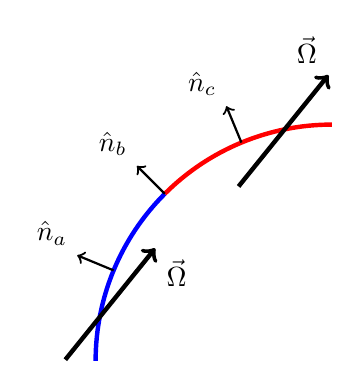
\begin{tikzpicture}
\draw[blue, ultra thick] (-3,0) arc (180:135:3);
\draw[red, ultra thick] (-2.1213,2.1213) arc (135:90:3);

\draw[->,thick] (-2.7716,1.1481) -- (-3.2336,1.3394) node[anchor=south east]{$\hat{n}_a$};
\draw[->,thick] (-2.1213,2.1213) -- (-2.4749,2.4749) node[anchor=south east]{$\hat{n}_b$};
\draw[->,thick] (-1.1481,2.7716) -- (-1.3394,3.2336) node[anchor=south east]{$\hat{n}_c$};

\draw[black,->,ultra thick] (-3.3848,0.0142) -- (-2.2436,1.4284) node[anchor=north west]{$\vec{\Omega}$};
\draw[black,->,ultra thick] (-1.1848,2.2142) -- (-0.0436,3.6284) node[anchor=south east]{$\vec{\Omega}$};

\end{tikzpicture}
\caption{Example of an incident and outgoing surface.}
\label{fig:IncidentOutgoingSurface}
\end{figure}
%
The blue portion represents an incident flux because $\vec{\Omega} \vd \hat{n}_a < 0$. The $P^+$ numerical integration is performed along the entire surface but only the integration points on the blue portion are nonzero. The red portion represents an outgoing flux because $\vec{\Omega} \vd \hat{n}_c > 0$. The $P^-$ numerical integration is performed along the entire surface but only the integration points on the red portion are nonzero. The default integration order is $\mathcal{Q} = 2p+d \cdot g -1$ along the surface $\partial \mathcal{D}_k^i$, where $d$ is the dimension of the spatial domain (this research uses $d=2$) and $g$ is the order of the mesh zone.

Substituting Equation~\ref{eq:xySplitUpwind} into Equation~\ref{eq:IntegrateByParts}, we have
\begin{multline}
- \left(\vec{\Omega}_m \vd \grad v_{ki}, \psi_m \right)_{\mathcal{D}_k} + \left(\sigma_t\ \psi_m, v_{ki} \right)_{\mathcal{D}_k} + \sum_{\partial \mathcal{D}_k^b} \left(\vec{\Omega}_m \vd \hat{n}\ \mathcal{I}_m^-, v_{ki} \right)_{\partial \mathcal{D}_k^b} \\
+ \sum_{\partial \mathcal{D}_k^i} \left(\vec{\Omega}_m \vd \hat{n}\ \mathcal{I}_m^+, v_{ki} \right)_{\partial \mathcal{D}_k^i} + \sum_{\partial \mathcal{D}_k^i} \left(\vec{\Omega}_m \vd \hat{n}\ \mathcal{I}_m^-, v_{ki} \right)_{\partial \mathcal{D}_k^i} \\
= \frac{1}{4 \pi} \left(\sigma_s\ \phi, v_{ki} \right)_{\mathcal{D}_k} + \frac{1}{4 \pi} \left(S_0, v_{ki} \right)_{\mathcal{D}_k} + \sum_{\partial \mathcal{D}_k^b} \left(\left| \vec{\Omega}_m \vd \hat{n} \right| \mathcal{I}_m^b, v_{ki} \right)_{\partial \mathcal{D}_k^b}.
\label{eq:FinalDFEM}
\end{multline}

\noindent Here we computed the boundary surface terms using the same approach as for interior surfaces, with a known boundary condition $\mathcal{I}_m^+ \equiv \mathcal{I}_m^b$ as the upwind value. If we performed a transport sweep (spatial sweep) through the mesh, the known (previously computed) upwind values $\psi_m^+$ would be used in the  $\mathcal{I}_m^+$ term and subtracted to the right-hand-side. Since we generate a matrix that contains all spatial degrees of freedom, we leave this term in the bilinear form. These upstream values are dependent upon the degrees of freedom in each neighboring mesh zone. Thus, our global matrix contains off-diagonal sub-matrices that contain these couplings between mesh zones.

We assume the unknown angular and scalar fluxes in each mesh zone can be expanded in terms of basis functions $\varphi(\vec{r})$,
\begin{flalign}
\psi (\vec{x}, \vec{\Omega}_m) & \approx \sum_{j=1}^{L_k} \psi_{kj} (\vec{\Omega}_m)\ \varphi_{kj} (\vec{x}), \quad \vec{x} \in \mathcal{D}_k, \\
\phi (\vec{x}) & \approx \sum_{j=1}^{L_k} \phi_{kj}\ \varphi_{kj}(\vec{x}), \quad \vec{x} \in \mathcal{D}_k
\end{flalign}

\noindent for basis functions $j=1, \dots, L_k$, for $L_k$ basis functions in mesh zone $k$. We use the standard Galerkin finite element method, in which the basis functions are equal to the test (weight) functions~\cite{ErnGuermond}.

We employ Lagrange basis functions --- the function equals unity at the integration point they ``live'' on and zero at all of the others. In two-dimensions, the general form of the first-order polynomial basis function is
\begin{flalign}
b(x,y) & = a x y + b x + c y + d,
\end{flalign}
%
and the second-order basis function,
\begin{flalign}
b(x,y) & = a x^2 y^2 + b x^2 y + c x^2 + d x y^2 + e x y + f x + g y^2 + h y + j,
\end{flalign}
%
where the sets $\{a,b,c,d\}$ and $\{a,b,c,d,e,f,g,h,j\}$ are the sets of coefficients that define the unique basis function for each integration point, respectively. This same methodology applies to higher-order basis functions. The location of the integration points is important. For example, we may place these evenly across the reference element or at Gauss-Legendre quadrature locations. On the unit square $[0,1] \times [0,1]$, the Gauss-Legendre integration points are located at the cross product of the nodes on $[0,1]$. Listed for linear, quadratic, and cubic finite elements in Table~\ref{tab:GaussianQuadrature}, the Gauss-Legendre integration point abscissas~\cite{Abramowitz1972Handbook} were transformed from the traditional $[-1,1]$ to the reference element length $[0,1]$.

\begin{table}[!htb]
\centering
{\renewcommand{\arraystretch}{2}
\begin{tabular}{|c|c|c|}
\hline
FE order & Points on $[-1,1]$ & Points on $[0,1]$ \\\hline
1 & $\displaystyle \pm \frac{1}{\sqrt{3}}$ & \begin{tabular}{c} $\displaystyle \frac{1}{3 + \sqrt{3}}$ \\ $\displaystyle 1- \frac{1}{3+\sqrt{3}}$ \end{tabular} \\\hline
2 & \begin{tabular}{c} 0 \\ $\displaystyle \pm \sqrt{\frac{3}{5}}$ \end{tabular} & \begin{tabular}{c} $\displaystyle \frac{1}{5 + \sqrt{15}}$ \\ 0.5 \\ $\displaystyle 1- \frac{1}{5+\sqrt{15}}$ \end{tabular} \\\hline
3 & \begin{tabular}{c} $\displaystyle \pm \sqrt{\frac{3}{7} - \frac{2}{7} \sqrt{\frac{6}{5}}}$ \\ $\displaystyle \pm \sqrt{\frac{3}{7} + \frac{2}{7} \sqrt{\frac{6}{5}}}$ \end{tabular} & \begin{tabular}{c} $\displaystyle \frac{10+\sqrt{30}}{35 + \sqrt{35(15-2 \sqrt{30})}}$ \\ $\displaystyle \frac{10-\sqrt{30}}{35 + \sqrt{35(15-2 \sqrt{30})}}$ \\ $\displaystyle 1- \frac{10+\sqrt{30}}{35 + \sqrt{35(15-2 \sqrt{30})}}$ \\ $\displaystyle 1- \frac{10-\sqrt{30}}{35 + \sqrt{35(15-2 \sqrt{30})}}$ \end{tabular} \\\hline
\end{tabular}}
\caption{Gaussian quadrature locations.}
\label{tab:GaussianQuadrature}
\end{table}

Once the finite element order and the set of integration points is determined, the linear system can be arranged to determine the coefficients. For example, to determine the first-order basis function that ``lives'' at integration point $(x_1, y_1)$ (and is equal to unity at that integration point and is zero at the remaining three), we assemble the system of equations
\begin{flalign}
\begin{bmatrix}
x_1 y_1 & x_1 & y_1 & 1 \\
x_2 y_2 & x_2 & y_2 & 1 \\
x_3 y_3 & x_3 & y_3 & 1 \\
x_4 y_4 & x_4 & y_4 & 1
\end{bmatrix}
\begin{bmatrix}
a \\
b \\
c \\
d
\end{bmatrix}
& =
\begin{bmatrix}
1 \\
0 \\
0 \\
0
\end{bmatrix}.
\end{flalign}
%
The 1 inside the solution vector on the right-hand-side determines which basis function coefficients will be obtained. For example, the right-hand-side vector $\left[0,0,1,0 \right]^T$ will return the basis function coefficients for the third integration point at $(x_3, y_3)$.

%%%%%%%%%%%%%%%%%%%%%%%%%%%%%%%%%%%%%%%
\subsection{Meshes with Curved Surfaces}
\label{sec:HOMeshes}
The basis functions are spatially dependent. Therefore, they are unique to each physical mesh zone due to the shape and location of each zone. We avoid having to perform calculations with arbitrarily large set of basis functions by utilizing the reference element and transforming the reference element into the physical element. We employ the same reference element for each mesh zone, where the basis functions are identical regardless of the physical element shape and position. After performing the DFEM integrations, we transform the solution from the reference element to the physical element. Each mesh zone will have a unique transformation but an identical set of basis functions to obtain the solution on the reference element. In general, the basis functions are allowed to be unique to each element, but we use the same set of basis functions across all elements for simplicity.

We can perform arbitrary-order mapping, preserving arbitrary-order curved mesh elements. To demonstrate, we provide an example bi-quadratic mapping. Figure~\ref{fig:HOMapping} shows the bi-quadratic mapping from the reference element to a physical element and has the following functional form
\begin{flalign}
\begin{bmatrix}
x(\lambda, \kappa) \\
y(\lambda, \kappa)
\end{bmatrix}
& = \sum_{i=1}^{J_k} \sum_{j=1}^{J_k}
\begin{bmatrix}
x_{ij} \\
y_{ij}
\end{bmatrix}
N_i(\lambda) N_j(\kappa)
\label{eq:MeshMappingFuncForm}
\end{flalign}
%
where
\begin{flalign}
N_l(\chi) & =
\begin{cases}
(2\chi-1)(\chi-1), & l = 1 \\
4\chi(1-\chi), & l = 2 \\
\chi(2\chi-1), & l = 3
\end{cases}
\label{eq:BiQuadMeshMapping}
\end{flalign}
%
are the quadratic basis functions that have support points at typical vertices shown in the left image of Figure~\ref{fig:HOMapping}.
%
\begin{figure}[!htb]
\centering
\hspace{-25pt}
\begin{minipage}[c]{7.25cm}
\raggedleft
\begin{tikzpicture}
\begin{axis}[
	axis lines=left,
	width=6.5cm,
	height=6.5cm,
    xmin=0, xmax=1,
    ymin=0, ymax=1,
    xlabel={$\lambda$},
    ylabel={$\kappa$},
    ]
    \addplot[only marks, mark=*, mark size=1, color=blue, mark options={solid, fill=blue}] table [x index=0, y index=1]{./graphics/MeshReference.dat};
    \addplot[only marks, mark=*, mark size=3, color=black, mark options={solid, fill=black}] table [x index=0, y index=1]{./graphics/MeshNodes.dat};
\end{axis}
\end{tikzpicture}
\end{minipage}
\begin{minipage}[c]{0.75cm}
\centering
{\Huge$\mapsto$}
\end{minipage}
\begin{minipage}[c]{7.5cm}
\raggedright
\begin{tikzpicture}
\begin{axis}[
	axis lines=left,
	width=6.5cm,
	height=6.5cm,
    xmin=0.9, xmax=2.5,
    ymin=0.8, ymax=2.5,
    xlabel={$x$},
    ylabel={$y$},
    ]
    \addplot[only marks, mark=*, mark size=1, color=red, mark options={solid, fill=red}] table [x index=0, y index=1]{./graphics/MeshTransform.dat};
    \addplot[only marks, mark=*, mark size=3, color=black, mark options={solid, fill=black}] table [x index=0, y index=1]{./graphics/MeshTransNodes.dat};
\end{axis}
\end{tikzpicture}
\end{minipage}
\caption{Example of mapping the reference element to a physical element.}
\label{fig:HOMapping}
\end{figure}
%
The $(x_{ij}, y_{ij})$ coordinates are the locations of the vertices in the physical element and are generally known.  Equations~\ref{eq:MeshMappingFuncForm}~and~\ref{eq:BiQuadMeshMapping} determine the $(x,y)$ coordinates for each $(\lambda, \kappa)$ vertex in the reference element. For example, the physical element vertex $(x_{12},y_{12})=(1.25,1.4)$ is the location on the physical zone that is mapped from $(\lambda,\kappa)=(0,0.5)$ on the reference element. That is,
\begin{flalign}
x(0,0.5) & = 1.25, \text{ and} \\
y(0,0.5) & = 1.4.
\end{flalign}

The determinant of the Jacobian of the transformation,
\begin{flalign}
\det \left[J(\lambda, \kappa) \right] & =
{\renewcommand{\arraystretch}{1.5}
\begin{vmatrix}
\dfrac{\partial x(\lambda,\kappa)}{\partial \lambda} & \dfrac{\partial y(\lambda,\kappa)}{\partial \lambda} \\
\dfrac{\partial x(\lambda,\kappa)}{\partial \kappa} & \dfrac{\partial y(\lambda,\kappa)}{\partial \kappa}
\end{vmatrix}},
\label{eq:DeterminantJacobian}
\end{flalign}
%
is used to perform the mapping from the physical space to $\lambda$-$\kappa$ space. We perform the coordinate transformation from the reference element using the determinant of the Jacobian of the mapping and evaluate numerically. For example, applied to Equation~\ref{eq:InnerProductNotation}, this mapping is
\begin{subequations}
\begin{flalign}
\int_{\mathcal{D}_k} a(x,y)\ b(x,y)\ dx\ dy & = \int_0^1 d \kappa \int_0^1 d \lambda\ a(\lambda,\kappa)\ b(\lambda,\kappa)\ \det (J(\lambda,\kappa)) \\
& \approx \sum_{i,j}^\mathcal{Q} w_i\ w_j\ a(\lambda_{i},\kappa_{j})\ b(\lambda_{i},\kappa_{j})\ \det(J(\lambda_{i},\kappa_{j})),
\end{flalign}
\label{eqs:InnerProductDetJac}
\end{subequations}

\noindent where $\lambda_{i}$ and $\kappa_{j}$ are Gauss-Legendre integration points with associated quadrature weights $w_{i}$ and $w_{j}$, and $\mathcal{Q}$ is large enough to exactly integrate the polynomials. The default integration order we used is $\mathcal{Q}=2p+d g-1$, where $p$ is the finite element order, $d$ is the number of spatial dimensions, and $g$ is the order of the mesh.

%%%%%%%%%%%%%%%%%%%%%%%%%%%%%%%%%%%%%%%
\subsection{Solution Method}
\label{sec:SolutionMethod}
This section falls within the ``Radiation transport solve'' and ``Update scalar flux'' steps of Figure~\ref{fig:SolutionFlowDiagram}. We employ the Modular Finite Elements Library (MFEM)\footnote{\url{mfem.org}} to perform integrations to assemble the system of equations for each element. These elements are then assembled into a global matrix that acts on each spatial degree of freedom simultaneously.

The meshes described in Section~\ref{sec:HOMeshes} add complexities to the numerical methods used to solve the transport equation. It is common to solve for a single mesh zone using incident angular flux information and propagate that angular flux from mesh zone to mesh zone, sweeping through the grid~\cite{Pautz2002ParallelSweeps,WareingDFEM3DUnsGrid}. However, if any particular mesh zone has both incident and outgoing angular fluxes to another mesh zone, they depend upon each other in a cyclic manner. ``Breaking the cycle'' is some fashion is necessary to perform the numerical computation. Instead of sweeping through the grid, we utilize MFEM to assemble each local element system of equations into a global system of equations, where the inter-element dependencies appear as off-diagonal block matrices. This global system of equations solves for all spatial degrees of freedom within all mesh zones for the entire problem. This is computationally intensive, but it bypasses the need to consider any cycles that may occur. The goal of this work is to evaluate the methodology, not solution efficiency.

After generating the system of equations, we use UMFPack, a direct solver that performs a LU decomposition~\cite{SuiteSparse, DavisUMFPack} to solve for all of the spatial degrees of freedom for direction $\vec{\Omega}_m$. This satisfies the ``End of \emph{m} loop'' criterion of Figure~\ref{fig:SolutionFlowDiagram}. We solve the global system of equations for the scalar flux, $\phi$, using either the source iteration method (SI) (Equations~\ref{eqs:SourceIteration} and ``Update scalar flux'' of Figure~\ref{fig:SolutionFlowDiagram}) or the DSA SI (Equations~\ref{eq:DSASITransport},~\ref{eq:DSASIPhiHalf}, and~\ref{eqs:DSAAlgorithm}, and both ``DSA solve'' and ``Update scalar flux'' within Figure~\ref{fig:SolutionFlowDiagram}). The iterative process continues until the convergence criterion
\begin{flalign}
\norm{\phi^{\left(\ell+1 \right)} - \phi^{\left(\ell \right)}}_\infty < \varepsilon_\text{conv} \left(1 - \rho_\text{sr} \right) \norm{\phi^{\ell+1}}_\infty,
\label{eq:ConvergenceCriteria}
\end{flalign}

\noindent is met, where $\varepsilon_\text{conv}$ is some small tolerance, $\rho_\text{sr}$ is the estimated spectral radius,
\begin{flalign}
\rho_\text{sr} & \approx \frac{\norm{\phi^{(\ell+1)} - \phi^{(\ell)}}_\infty}{\norm{\phi^{(\ell)} - \phi^{(\ell-1)}}_\infty},
\label{eq:SpectralRadius}
\end{flalign}
%
\noindent as described by Adams and Larsen~\cite{AdamsFastIterativeMethods}, and where
\begin{flalign}
\norm{\vec{y}}_\infty & = \max_i (y_i).
\end{flalign}

\noindent This satisfies the ``Scalar flux converged'' criterion of Figure~\ref{fig:SolutionFlowDiagram}. The spectral radius is the measure of the convergence rate during the source iteration. This convergence criterion protects against false convergence. That is, for slowly converging solutions, two sequential scalar fluxes may be sufficiently similar, appearing to be converged. The spectral radius is used in the convergence criterion to signal the slow convergence and prevent the false indication that the scalar flux has converged. We initiated all of the iterative solves with an initial scalar flux at each integration point randomly varying between $-1000$ and $+1000$.

%%%%%%%%%%%%%%%%%%%%%%%%%%%%%%%%%%%%%%%
\subsection{\RZ\ Geometry}
\label{sec:MethodsRZ}
This section falls within the ``Spatial discretization'' step of Figure~\ref{fig:SolutionFlowDiagram}. Solving the transport equation in different coordinate systems may provide simpler ways of modeling a particular geometry or symmetry. In this section, we derive the \RZ\ transport equation to be solved. Section~\ref{sec:RZGeometryIntro} contains the introduction to the streaming operator in \RZ\ geometry. Some of that work is reproduced here for completeness.

The streaming operator in \RZ\ geometry is~\cite{Lewis_Comp_Methods_Neu_Trans}
\begin{flalign}
\vec{\Omega} \vd \grad \psi & = \frac{\mu}{r} \frac{\partial}{\partial r} (r \psi) + \xi \frac{\partial \psi}{\partial z} - \frac{1}{r} \frac{\partial}{\partial \omega} (\eta \psi),
\tag{\ref{eq:RZStreamingTerm}}
\end{flalign}
%
where $\vec{\Omega}$ is the direction-of-travel unit vector, $\psi$ is the angular flux, and
\begin{flalign}
\mu & \equiv \vec{\Omega} \vd \hat{e}_\mu = \sqrt{1 - \xi^2} \cos \omega = \sin(\theta) \cos(\omega), \tag{\ref{eq:muDef}} \\
\eta & \equiv \vec{\Omega} \vd \hat{e}_\eta = \sqrt{1 - \xi^2} \sin \omega = \sin(\theta) \sin(\omega), \tag{\ref{eq:etaDef}} \\
\xi & \equiv \vec{\Omega} \vd \hat{e}_\xi = \cos(\theta). \tag{\ref{eq:xiDef}}
\end{flalign}
%
The variables $\mu$, $\eta$, $\xi$, $\omega$, and $\theta$ are shown in the cylindrical coordinate system in Figure~\ref{fig:CylindricalCoordinateSystem}. The key point is that the coordinate system describing $\vec{\Omega}$ depends upon the spatial position. The steady-state, mono-energetic transport equation in \RZ\ geometry is then
\begin{multline}
\frac{\mu}{r} \frac{\partial}{\partial r} r \psi \left(r,z, \vec{\Omega} \right) + \xi \frac{\partial}{\partial z} \psi \left(r,z,\vec{\Omega} \right) - \frac{1}{r} \frac{\partial}{\partial \omega} \eta \psi \left(r,z, \vec{\Omega} \right) + \sigma_t \left(r,z \right) \psi \left(r,z,\vec{\Omega} \right) \\
= \frac{1}{4 \pi} \sigma_s \left(r,z \right) \phi \left(r,z \right) + S_0 \left(r,z, \vec{\Omega} \right).
\label{eq:RZTransport}
\end{multline}

We divide the angular-spatial discretizations into two sections. In Section~\ref{sec:RZAngularDiscretization}, we discretize the \RZ\ transport equation using the discrete ordinates method. In Section~\ref{sec:RZSpatialDiscretization}, we perform the discretization of the spatial domain using HO DFEM.

%%%%%%%%%%%%%%%%%%%%%%%%%%%%%%%%%%%%%%%
\subsubsection{Angular Discretization}
\label{sec:RZAngularDiscretization}
This section falls within the ``Angular discretization'' step of Figure~\ref{fig:SolutionFlowDiagram}. Discretizing Equation~\ref{eq:RZTransport} with a level-symmetric angular quadrature results in 
\begin{multline}
\frac{\mu_{n,m}}{r} \frac{\partial}{\partial r} r \psi_{n,m} \left(r,z \right) + \xi_n \frac{\partial}{\partial z} \psi_{n,m} \left(r,z \right) - \frac{1}{r} \frac{\partial}{\partial \omega} \eta_{n,m} \psi_{n,m} \left(r,z \right) + \sigma_t \left(r,z \right) \psi_{n,m} \left(r,z \right) \\
= \frac{1}{4 \pi} \int_{4 \pi} \sigma_s \left(r,z \right) \phi \left(r,z, \vec{\Omega}^\prime \right) d \Omega^\prime + S_0 \left(r,z, \vec{\Omega} \right)
\label{eq:RZSNTransport}
\end{multline}

\noindent for direction $\vec{\Omega}_{n,m}$, where index $n$ describes a level of quadrature with constant $\xi$ and the $m$ index denotes the quadrature point on that level. The $(n,m)$ indexing is shown in Figure~\ref{fig:AngularDiscretization}.

\begin{figure}[!htb]
\centering
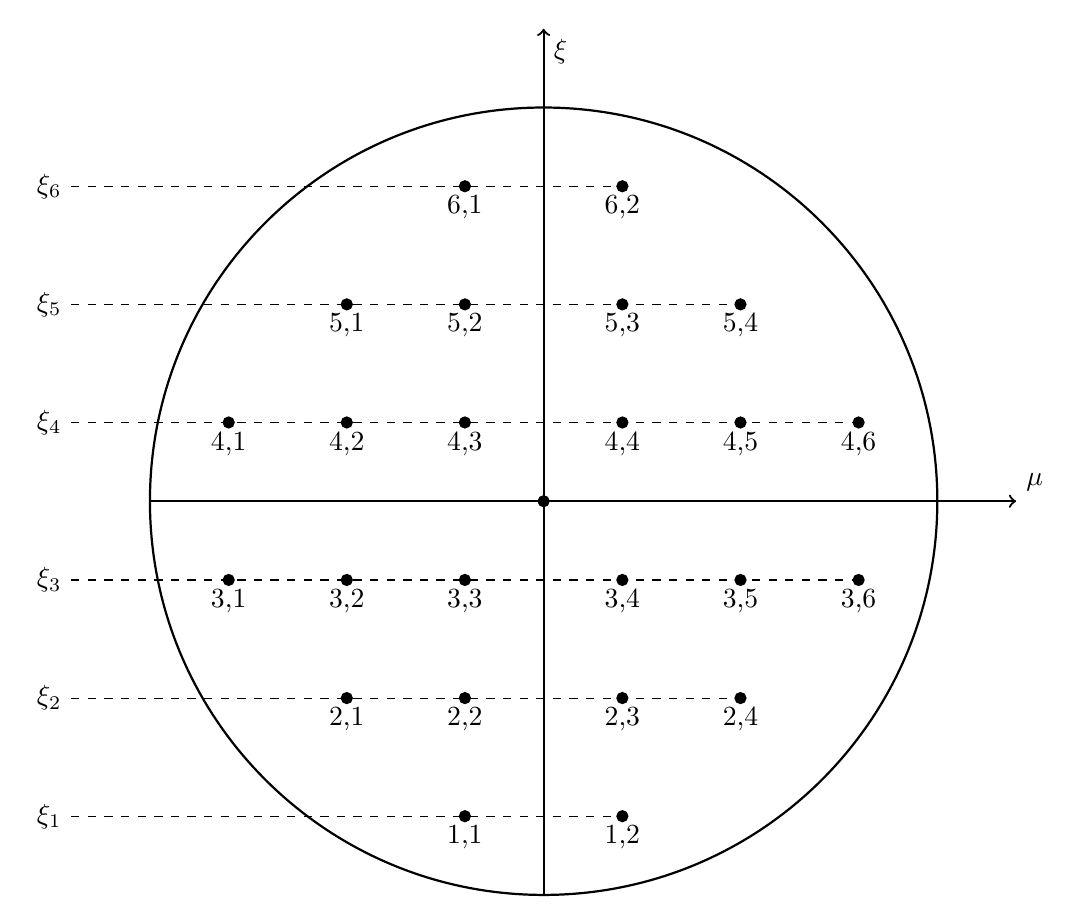
\begin{tikzpicture}

\draw[fill=black] (0,0) circle (2pt);
\draw[thick,->] (-5,0) -- (6,0) node[above right]{$\mu$};
\draw[thick,->] (0,-5) -- (0,6) node[below right]{$\xi$};
\draw[thick] (0,0) circle (5cm);

\draw[dashed] (-6,-4) node[left]{$\xi_1$} -- (1,-4);
\draw[dashed] (-6,-2.5) node[left]{$\xi_2$} -- (2.5,-2.5);
\draw[dashed] (-6,-1) node[left]{$\xi_3$} -- (4,-1);
\draw[dashed] (-6,1) node[left]{$\xi_4$} -- (4,1);
\draw[dashed] (-6,2.5) node[left]{$\xi_5$} -- (2.5,2.5);
\draw[dashed] (-6,4) node[left]{$\xi_6$} -- (1,4);

\draw[fill=black] (-4,-1) circle (2pt) node[below]{3,1};
\draw[fill=black] (-2.5,-1) circle (2pt) node[below]{3,2};
\draw[fill=black] (-1,-1) circle (2pt) node[below]{3,3};
\draw[fill=black] (-2.5,-2.5) circle (2pt) node[below]{2,1};
\draw[fill=black] (-1, -2.5) circle (2pt) node[below]{2,2};
\draw[fill=black] (-1,-4) circle (2pt) node[below]{1,1};

\draw[fill=black] (1,-1) circle (2pt) node[below]{3,4};
\draw[fill=black] (2.5,-1) circle (2pt) node[below]{3,5};
\draw[fill=black] (4,-1) circle (2pt) node[below]{3,6};
\draw[fill=black] (1, -2.5) circle (2pt) node[below]{2,3};
\draw[fill=black] (2.5,-2.5) circle (2pt) node[below]{2,4};
\draw[fill=black] (1,-4) circle (2pt) node[below]{1,2};

\draw[fill=black] (-4,1) circle (2pt) node[below]{4,1};
\draw[fill=black] (-2.5,1) circle (2pt) node[below]{4,2};
\draw[fill=black] (-1,1) circle (2pt) node[below]{4,3};
\draw[fill=black] (-2.5,2.5) circle (2pt) node[below]{5,1};
\draw[fill=black] (-1, 2.5) circle (2pt) node[below]{5,2};
\draw[fill=black] (-1,4) circle (2pt) node[below]{6,1};

\draw[fill=black] (1,1) circle (2pt) node[below]{4,4};
\draw[fill=black] (2.5,1) circle (2pt) node[below]{4,5};
\draw[fill=black] (4,1) circle (2pt) node[below]{4,6};
\draw[fill=black] (1, 2.5) circle (2pt) node[below]{5,3};
\draw[fill=black] (2.5,2.5) circle (2pt) node[below]{5,4};
\draw[fill=black] (1,4) circle (2pt) node[below]{6,2};

\end{tikzpicture}
\caption{Angular discretization showing $(\xi,\mu)$ pairs; adapted from~\cite{Lewis_Comp_Methods_Neu_Trans}}
\label{fig:AngularDiscretization}
\end{figure}

One of the major challenges is handling the anglar derivative term. Lewis and Miller~\cite{Lewis_Comp_Methods_Neu_Trans} describes an approximation for the partial derivative of the angular flux with respect to $\omega$:
\begin{flalign}
- \frac{1}{r} \frac{\partial}{\partial \omega} \eta_{m,n} \psi_{n,m} \left(r,z \right) & = \frac{\alpha_{m+1/2}^n \psi_{n,m+1/2} (r,z) - \alpha_{m-1/2}^n \psi_{n,m-1/2} (r,z)}{r w_{n,m}}
\end{flalign}

\noindent where $\alpha_{m+1/2}^n$ and $\alpha_{m-1/2}^n$ are angular differencing coefficients, $\psi_{n,m+1/2}$ and $\psi_{n,m-1/2}$ are the angular fluxes in the $(\xi_n,\mu_{n,m+1/2})$- and $(\xi_n,\mu_{n,m-1/2})$-directions, respectively, and $w_{n,m}$ is the angular quadrature weight. We substitute this into Equation~\ref{eq:RZSNTransport},
\begin{multline}
\frac{\mu_{n,m}}{r} \frac{\partial}{\partial r} r \psi_{n,m} \left(r,z \right) + \xi_n \frac{\partial}{\partial z} \psi_{n,m} \left(r,z \right) \\
+ \frac{\alpha_{m+1/2}^n \psi_{n,m+1/2} (r,z) - \alpha_{m-1/2}^n \psi_{n,m-1/2} (r,z)}{r w_{n,m}} + \sigma_t \left(r,z \right) \psi_{n,m} \left(r,z \right) \\
= \frac{1}{4 \pi} \int_{4 \pi} \sigma_s \left(r,z \right) \psi \left(r,z, \vec{\Omega}^\prime \right) d \Omega^\prime + \frac{1}{4 \pi} S_0 \left(r,z \right)
\label{eq:RZSNADTransport}
\end{multline}

\noindent Here, we pause to notice that there are similarities and differences between a Cartesian discretization. The absorption term, axial derivative term, and right-hand-side are the same in both coordinate systems. The differences arise in the radial and angular derivative terms.

Requiring Equation~\ref{eq:RZSNADTransport} to satisfy the uniform infinite medium solution results in the condition,
\begin{flalign}
\alpha_{m+1/2}^n & = \alpha_{m-1/2}^n - \mu_{n,m} w_{n,m}
\label{eq:AlphaMinusMuW}
\end{flalign}

\iffalse
\begin{multline}
\int_{4 \pi} d \Omega \left[ \frac{\mu_{n,m}}{r} \frac{\partial}{\partial r} r \psi_{n,m} \left(r,z \right) + \frac{\alpha_{m+1/2}^n \psi_{m+1/2,n} (r,z) - \alpha_{m-1/2}^n \psi_{m-1/2,n} (r,z)}{r w_{n,m}} \right. \\
\left. + \xi_n \frac{\partial}{\partial z} \psi_{n,m} \left(r,z \right) \right] + \sigma_t \left(r,z \right) \phi \left(r,z \right) \\
= \sigma_s \left(r,z \right) \phi \left(r,z\right) + S_0 \left(r,z \right)
\end{multline}
\begin{multline}
\int_{4 \pi} d \Omega \left[ \frac{\mu_{n,m}}{r} \frac{\partial}{\partial r} r \psi_{n,m} \left(r,z \right) + \frac{\alpha_{m+1/2}^n \psi_{m+1/2,n} (r,z) - \alpha_{m-1/2}^n \psi_{m-1/2,n} (r,z)}{r w_{n,m}} \right. \\
\left. + \xi_n \frac{\partial}{\partial z} \psi_{n,m} \left(r,z \right) \right] = 0
\end{multline}

\noindent That is, the streaming term must equal zero because $\sigma_t = \sigma_a + \sigma_s$. Using the product rule,
\begin{multline}
\int_{4 \pi} d \Omega \left[\frac{\mu_{n,m}}{r} \left(\frac{\partial r}{\partial r} \psi_{n,m} + r \frac{\partial \psi_{n,m} (r,z)}{\partial r} \right) + \right. \\
\left. \frac{\alpha_{m+1/2}^n \psi_{m+1/2,n} (r,z) - \alpha_{m-1/2}^n \psi_{m-1/2,n} (r,z)}{r w_{n,m}} + \xi_n \frac{\partial}{\partial z} \psi_{n,m} \left(r,z \right) \right] = 0
\end{multline}
\begin{flalign}
\int_{4 \pi} d \Omega \left[\frac{\mu_{n,m}}{r} \psi_{n,m} + \frac{\alpha_{m+1/2}^n \psi_{m+1/2,n} (r,z) - \alpha_{m-1/2}^n \psi_{m-1/2,n} (r,z)}{r w_{n,m}} \right] & = 0 \\
\left(\frac{\mu_{n,m}}{r} + \frac{\alpha_{m+1/2}^n - \alpha_{m-1/2}^n}{r w_{n,m}} \right) \phi(r,z) & = 0
\end{flalign}

\noindent results in the condition,
\begin{flalign}
\alpha_{m+1/2}^n & = \alpha_{m-1/2}^n - \mu_{n,m} w_{n,m}
\label{eq:AlphaMinusMuW}
\end{flalign}
\fi

\noindent If $\alpha_{1/2}^n$ is known, then the remaining coefficients are uniquely determined. To find $\alpha_{1/2}^n$, we require that the angular flux of Equation~\ref{eq:RZSNADTransport} also satisfy the conservation equation (Equation~\ref{eq:RZTransport}).
%
\iffalse
Discretizing Equation~\ref{eq:RZTransport} using discrete ordinates and summing over all directions (approximately integrating over all directions),
\begin{multline}
\sum_{n=1}^N \sum_{m=1}^{M_n} \frac{1}{r} \frac{\partial}{\partial r} r w_{n,m} \mu_{n,m} \psi_{n,m} \left(r,z \right) - \sum_{n=1}^N \sum_{m=1}^{M_n} \frac{1}{r} \frac{\partial}{\partial \omega} w_{n,m} \eta_{n,m} \psi_{n,m} \left(r,z \right) \\
+ \sum_{n=1}^N \sum_{m=1}^{M_n} \xi_n \frac{\partial}{\partial z} w_{n,m} \psi_{n,m} \left(r,z \right) + \sum_{n=1}^N \sum_{m=1}^{M_n} \sigma_t \left(r,z \right) \psi_{n,m} \left(r,z \right) \\
= \sum_{n=1}^N \sum_{m=1}^{M_n} w_{n,m} \frac{1}{4 \pi} \int_{4 \pi} \sigma_s \left(r,z \right) \psi \left(r,z, \vec{\Omega}^\prime \right) d \Omega^\prime + \sum_{n=1}^N \sum_{m=1}^{M_n} w_{n,m} \frac{1}{4 \pi} S_0 \left(r,z \right)
\end{multline}

\noindent Given that the sum of the weights is $\sum w = 4 \pi$,
\begin{multline}
\sum_{n=1}^N \sum_{m=1}^{M_n} \frac{1}{r} \frac{\partial}{\partial r} r w_{n,m} \mu_{n,m} \psi_{n,m} \left(r,z \right) - \sum_{n=1}^N \sum_{m=1}^{M_n} \frac{1}{r} \frac{\partial}{\partial \omega} w_{n,m} \eta_{n,m} \psi_{n,m} \left(r,z \right) \\
+ \sum_{n=1}^N \sum_{m=1}^{M_n} \xi_n \frac{\partial}{\partial z} w_{n,m} \psi_{n,m} \left(r,z \right) \\
= - \sum_{n=1}^N \sum_{m=1}^{M_n} \sigma_t \left(r,z \right) \psi_{n,m} \left(r,z \right) + \int_{4 \pi} \sigma_s \left(r,z \right) \psi \left(r,z, \vec{\Omega}^\prime \right) d \Omega^\prime +  S_0 \left(r,z \right)
\end{multline}

\noindent Multiplying Equation~\ref{eq:RZSNADTransport} by weight $w_{n,m}$ and summing over all directions results in
\begin{multline}
\sum_{n=1}^N \sum_{m=1}^{M_n} w_{n,m} \frac{\mu_{n,m}}{r} \frac{\partial}{\partial r} r \psi_{n,m} \left(r,z \right) + \sum_{n=1}^N \sum_{m=1}^{M_n} w_{n,m} \frac{\alpha_{m+1/2}^n \psi_{m+1/2,n} (r,z) - \alpha_{m-1/2}^n \psi_{m-1/2,n} (r,z)}{r w_{n,m}} \\
+ \sum_{n=1}^N \sum_{m=1}^{M_n} w_{n,m} \xi_n \frac{\partial}{\partial z} \psi_{n,m} \left(r,z \right) + \sum_{n=1}^N \sum_{m=1}^{M_n} w_{n,m} \sigma_t \left(r,z \right) \psi_{n,m} \left(r,z \right) \\
= \sum_{n=1}^N \sum_{m=1}^{M_n} w_{n,m} \frac{1}{4 \pi} \int_{4 \pi} \sigma_s \left(r,z \right) \psi \left(r,z, \vec{\Omega}^\prime \right) d \Omega^\prime + \sum_{n=1}^N \sum_{m=1}^{M_n} w_{n,m} \frac{1}{4 \pi} S_0 \left(r,z \right)
\end{multline}

\noindent Then, to satisfy the condition,
\begin{multline}
- \sum_{n=1}^N \sum_{m=1}^{M_n} w_{n,m} \frac{1}{r} \frac{\partial}{\partial \omega} \eta_{n,m} \psi_{n,m} \left(r,z \right) \\
= \sum_{n=1}^N \sum_{m=1}^{M_n} w_{n,m} \frac{\alpha_{m+1/2}^n \psi_{m+1/2,n} (r,z) - \alpha_{m-1/2}^n \psi_{m-1/2,n} (r,z)}{r w_{n,m}}
\end{multline}
\begin{multline}
- \sum_{n=1}^N \sum_{m=1}^{M_n} w_{n,m} \left(\frac{\partial \eta_{n,m}}{\partial \omega} \psi_{n,m} \left(r,z \right) + \eta_{n,m} \frac{\partial \psi_{n,m} \left(r,z \right)}{\partial \omega} \right) \\
= \sum_{n=1}^N \sum_{m=1}^{M_n} \left(\alpha_{m+1/2}^n \psi_{m+1/2,n} (r,z) - \alpha_{m-1/2}^n \psi_{m-1/2,n} (r,z) \right)
\end{multline}

\noindent If $\int_{2 \pi} d \omega \frac{\partial}{\partial \omega} \eta \psi = 0$, then
\begin{flalign}
\sum_{m=1}^{M_n} \left(\alpha_{m+1/2}^n \psi_{m+1/2,n} (r,z) - \alpha_{m-1/2}^n \psi_{m-1/2,n} (r,z) \right) & = 0 \\
\alpha_{1/2}^n \psi_{1/2,n} (r,z) - \alpha_{M_n + 1/2}^n \psi_{M_n + 1/2,n} (r,z) & = 0
\end{flalign}
\fi
%
Given a quadrature set with an even number of $\mu_{n,m}$ values, setting $\alpha_{1/2}^n = 0$ results in $\alpha_{M_n + 1/2}^n = 0$ per Equation~\ref{eq:AlphaMinusMuW} and the conservation equation is satisfied.

\iffalse
 for any value of $\psi_{1/2,n} (r,z)$ and $\psi_{M_n + 1/2,n} (r,z)$.
\fi

A relationship between $\psi_{n,m}$, $\psi_{n,m+1/2}$, and $\psi_{n,m-1/2}$ must be established. A weighted diamond difference scheme has been established by Morel and Montry~\cite{MorelAnalysisEliminationFluxDip},
\begin{flalign}
\psi_{n,m} (r,z) & = \tau_{n,m} \psi_{n,m+1/2} + \left(1- \tau_{n,m} \right) \psi_{n,m-1/2},
\label{eq:LinearAngularFluxTau}
\end{flalign}

\noindent where $\tau_{n,m}$ linearly interpolates $\mu_{n,m}$:
\begin{flalign}
\tau_{n,m} & = \frac{\mu_{n,m} - \mu_{n,m-1/2}}{\mu_{n,m+1/2} - \mu_{n,m-1/2}},
\label{eq:LinearTau}
\end{flalign}

\noindent with
\begin{flalign}
\mu_{n,m+1/2} & = \sqrt{1 - \xi_n^2} \cos \left(\varphi_{n,m+1/2} \right), \\
\varphi_{n,m+1/2} & = \varphi_{n,m-1/2} + \pi \frac{w_{n,m}}{w_n}, \text{ and} \\
w_n & = \sum_{m=1}^{M_n} w_{n,m},
\end{flalign}

\noindent where $M_n$ is the number of discrete ordinate directions along $\xi_n$.

We multiply Equation~\ref{eq:RZSNADTransport} through by $r$ and perform a product rule on the $r$-derivative term,
\begin{multline}
\mu_{n,m} \left[\psi_{n,m} \left(r,z \right) + r \frac{\partial}{\partial r}  \psi_{n,m} \left(r,z \right) \right] + r \xi_n \frac{\partial}{\partial z} \psi_{n,m} \left(r,z \right) \\
+ \frac{\alpha_{m+1/2}^n \psi_{m+1/2,n} (r,z) - \alpha_{m-1/2}^n \psi_{m-1/2,n} (r,z)}{w_{n,m}} + r \sigma_t \left(r,z \right) \psi_{n,m} \left(r,z \right) \\
= \frac{r}{4 \pi} \int_{4 \pi} \sigma_s \left(r,z \right) \psi \left(r,z, \vec{\Omega}^\prime \right) d \Omega^\prime + \frac{r}{4 \pi} S_0 \left(r,z \right).
\end{multline}
%
We solve Equation~\ref{eq:LinearAngularFluxTau} for $\psi_{n,m+1/2}$, perform a substitution, and move the known quantities to the right-hand-side,
\begin{multline}
\setlength{\jot}{18pt}
\mu_{n,m} r \frac{\partial}{\partial r}  \psi_{n,m} \left(r,z \right) + r \xi_n \frac{\partial}{\partial z} \psi_{n,m} \left(r,z \right) + \mu_{n,m} \psi_{n,m} \left(r,z \right) \\
+ \frac{\alpha_{m+1/2}^n}{\tau_{n,m} w_{n,m}} \psi_{n,m}(r,z) + r \sigma_t \left(r,z \right) \psi_{n,m} \left(r,z \right) \\
= \frac{r}{4 \pi} \int_{4 \pi} \sigma_s \left(r,z \right) \psi \left(r,z, \vec{\Omega}^\prime \right) d \Omega^\prime + \frac{r}{4 \pi} S_0 \left(r,z \right) \\
+ \left(\frac{1-\tau_{n,m}}{\tau_{n,m}} \frac{\alpha_{m+1/2}^n}{w_{n,m}} + \frac{\alpha_{m-1/2}^n}{w_{n,m}} \right) \psi_{n,m-1/2}(r,z).
\label{eq:RZSNTransportFullAngular}
\end{multline}

Given a level-symmetric quadrature set, all of the $\alpha_{n,m \pm 1/2}^n$ and $\tau_{n,m}$ values can be computed. We solve the starting direction equation to obtain $\psi_{n,1/2}$. That is, we solve the \XY\ system for directions $\vec{\Omega}_{n,1/2}$,
\begin{flalign}
\vec{\Omega}_{n,1/2} \vd \grad \psi_{n,1/2} + \sigma_t \psi_{n,1/2} & = \frac{1}{4 \pi} \sigma_s \phi + \frac{1}{4 \pi} S_0
\end{flalign}

%%%%%%%%%%%%%%%%%%%%%%%%%%%%%%%%%%%%%%%
\subsubsubsection{Reflecting Boundary at $r=0$}
\label{sec:RZReflectingBoundary}
The angular flux at $r=0$ is a reflecting boundary --- there is rotational symmetry around the $z$-axis. This arises naturally in the analytic transport equation. Beginning with Equation~\ref{eq:RZTransport}, we multiply through by $r$, perform a product rule on the $r$-derivative term and set $r=0$. On the $z$-axis, the transport equation becomes
\begin{flalign}
\mu \psi - \frac{\partial}{\partial \omega} \left(\eta \psi \right) &= 0.
\end{flalign}

\noindent Then, performing a product rule on the angular derivative term results in,
\begin{flalign}
\mu \psi - \psi \frac{\partial \eta}{\partial \omega} - \eta \frac{\partial \psi}{\partial \omega} &= 0.
\end{flalign}

\noindent Since
\begin{flalign}
\frac{\partial \eta}{\partial \omega} \equiv \mu,
\end{flalign}

\noindent we can simplify this to
\begin{flalign}
\eta \frac{\partial \psi}{\partial \omega} = \eta \frac{\partial \psi}{\partial \mu} \frac{\partial \mu}{\partial \omega} = \eta^2 \frac{\partial \psi}{\partial \mu} & = 0. \\
\end{flalign}

\noindent Finally, we write
\begin{flalign}
\frac{\partial \psi}{\partial \omega} & = 0,
\end{flalign}

\noindent and
\begin{flalign}
\frac{\partial \psi}{\partial \mu} & = 0.
\label{eq:dpsidmu}
\end{flalign}

\noindent That is, the angular flux does not depend on $\omega$ (nor $\mu$) along the $z$-axis. Analytically, the transport equation has a naturally occurring reflecting boundary at $r=0$. This condition is also satisfied by the Morel and Montry discretization scheme. Beginning with Equation~\ref{eq:RZSNADTransport}, we multiply through by $r$, perform a product rule on the $r$-derivative term, and set $r=0$, resulting in
\begin{flalign}
\mu_{n,m} \psi_{n,m} + \frac{\alpha_{m+1/2}^n \psi_{n,m+1/2} - \alpha_{m-1/2}^n \psi_{n,m-1/2}}{w_{n,m}} & = 0.
\end{flalign}

\noindent We utilize the weighted diamond differencing relationship (Equation~\ref{eq:LinearAngularFluxTau}) to eliminate $\psi_{n,m+1/2}$ and rearrange:
\begin{flalign}
\left(\mu_{n,m} w_{n,m} \tau_{n,m} + \alpha_{m+1/2}^n \right) \psi_{n,m} & =  \left[\left(1-\tau_{n,m} \right) \alpha_{m+1/2}^n + \alpha_{m-1/2}^n \tau_{n,m} \right] \psi_{n,m-1/2}.
\end{flalign}

\noindent We also utilize Equation~\ref{eq:AlphaMinusMuW} and rearrange:
\begin{flalign}
\left(\mu_{n,m} w_{n,m} \tau_{n,m} + \alpha_{m+1/2}^n \right) \psi_{n,m} & =  \left(\alpha_{m+1/2}^n + \mu_{n,m} w_{n,m} \tau_{n,m} \right) \psi_{n,m-1/2}.
\end{flalign}

\noindent Finally, this simplifies to
\begin{flalign}
\psi_{n,m} & = \psi_{n,m-1/2},
\end{flalign}

\noindent which satisfies Equation~\ref{eq:dpsidmu}.

%%%%%%%%%%%%%%%%%%%%%%%%%%%%%%%%%%%%%%%
\subsubsection{Spatial Discretization}
\label{sec:RZSpatialDiscretization}
Here, we discretize the spatial domain using the discontinuous finite element method (DFEM). The methodology is similar to the Cartesian geometry (i.e., Section~\ref{sec:HODFEM}). First, we subdivide a problem domain using a spatial mesh. Then, we multiply Equation~\ref{eq:RZSNTransport} by a test function and integrate over the volume of mesh zone $\mathcal{D}_k$, dropping the arguments for brevity,
\begin{multline}
\left(r\ \vec{\Omega}_{n,m} \vd \left[\frac{\partial}{\partial r} \psi_{n,m} + \frac{\partial}{\partial z} \psi_{n,m} \right],\ v_{i} \right)_{\mathcal{D}_k} + \left(\mu_{n,m}\ \psi_{n,m},\ v_{i} \right)_{\mathcal{D}_k} \\
+ \left(r\ \sigma_t\ \psi_{n,m},\ v_{i} \right)_{\mathcal{D}_k} + \left(\frac{\alpha_{m+1/2}^n}{\tau_{n,m}\ w_{n,m}} \psi_{n,m},\ v_{i} \right)_{\mathcal{D}_k} \\
= \left(\frac{1}{4 \pi} r\ \sigma_s\ \phi,\ v_{i} \right)_{\mathcal{D}_k} + \left(\frac{1}{4 \pi} r\ S_0,\ v_{i} \right)_{\mathcal{D}_k} \\
+ \left(\left[\frac{\alpha_{m+1/2}^n}{w_{n,m}} \frac{(1-\tau_{n,m})}{\tau_{n,m}} + \frac{\alpha_{m-1/2}^n}{w_{n,m}} \right] \psi_{n,m-1/2},\ v_{i} \right)_{\mathcal{D}_k}
\end{multline}
%
where Equation~\ref{eq:ScalarFluxIntegral} and the inner product notation of Equation~\ref{eq:InnerProductNotation} have been used. We perform an integration by parts on the streaming term,
\begin{multline}
\sum_{\partial \mathcal{D}_k} \left(\vec{\Omega}_{n,m} \vd \hat{n}\ r\ \psi_{n,m}^\uparrow,\ v_{i} \right)_{\partial \mathcal{D}_k} - \left(r\ \psi_{n,m},\ \vec{\Omega}_{n,m} \vd \left[\frac{\partial}{\partial r} v_{i} + \frac{\partial}{\partial z} v_{i} \right] \right)_{\mathcal{D}_k} + \left(\mu_{n,m}\ \psi_{n,m},\ v_{i} \right)_{\mathcal{D}_k} \\
+ \left(r\ \sigma_t\ \psi_{n,m},\ v_{i} \right)_{\mathcal{D}_k} + \left(\frac{\alpha_{m+1/2}^n}{\tau_{n,m}\ w_{n,m}} \psi_{n,m},\ v_{i} \right)_{\mathcal{D}_k} \\
= \left(\frac{1}{4 \pi} r\ \sigma_s\ \phi,\ v_{i} \right)_{\mathcal{D}_k} + \left(\frac{1}{4 \pi} r\ S_0,\ v_{i} \right)_{\mathcal{D}_k} \\
+ \left(\left[\frac{\alpha_{m+1/2}^n}{w_{n,m}} \frac{(1-\tau_{n,m})}{\tau_{n,m}} + \frac{\alpha_{m-1/2}^n}{w_{n,m}} \right] \psi_{n,m-1/2},\ v_{i} \right)_{\mathcal{D}_k}
\end{multline}
%
\noindent to obtain the angular and spatially discretized \RZ\ transport equation, where $\partial \mathcal{D}_k$ is each of the surfaces on zone $\mathcal{D}_k$.

We perform numerical integrations to incorporate the mesh transformation from the reference element to the physical element by employing the determinant of the Jacobian defined by Equation~\ref{eq:DeterminantJacobian}. The general volume integrations are performed as described by Equations~\ref{eqs:InnerProductDetJac}.

The numerical integration of the surface term is more complicated. The sign of $\vec{\Omega}_{n,m} \vd \hat{n}(r,z)$ is evaluated at each spatial quadrature point along some surface $\partial \mathcal{D}_k$. Therefore, on a non-planar surface, the sign may switch between positive and negative denoting an outgoing or incident angular flux at the location of the quadrature point (see Figure~\ref{fig:IncidentOutgoingSurface} and surrounding text). Since we perform a Gaussian integration along each surface, we are approximating a continuous function that has a discontinuous first-derivative with a polynomial shape.

We apply the upwind approximation to the surface term
\begin{multline}
\sum_{\partial \mathcal{D}_k} \left(r \vec{\Omega}_{n,m} \vd \hat{n} \psi_{n,m}^\uparrow, v_{ki} \right)_{\partial \mathcal{D}_k} - \left(r \psi_{n,m}, \vec{\Omega}_{n,m} \vd \grad v_i \right)_{\mathcal{D}_k} + \left(\mu_{n,m} \psi_{n,m}, v_i \right)_{\mathcal{D}_k} \\
+ \left(\frac{\alpha_{m+1/2}^n}{\tau_{n,m} w_{n,m}} \psi_{n,m}, v_i \right)_{\mathcal{D}_k} + \left(r \sigma_t\psi_{n,m}, v_i \right)_{\mathcal{D}_k} \\
= \left(\frac{r}{4 \pi} \int_{4 \pi} \sigma_s \psi d \Omega^\prime, v_i \right)_{\mathcal{D}_k} + \left(\frac{r}{4 \pi} S_0, v_i \right)_{\mathcal{D}_k} \\
+ \left(\left(\frac{1-\tau_{n,m}}{\tau_{n,m}} \frac{\alpha_{m+1/2}^n}{w_{n,m}} + \frac{\alpha_{m-1/2}^n}{w_{n,m}} \right) \psi_{n,m-1/2}, v_i \right)_{\mathcal{D}_k},
\end{multline}

\noindent where
\begin{multline}
\sum_{\partial \mathcal{D}_k} \left(r\ \vec{\Omega}_{n,m} \vd \hat{n}(r,z)\ \psi_{n,m}^\uparrow, v_{ki} \right)_{\partial \mathcal{D}_k} \\
= \sum_{\partial \mathcal{D}_k^i} \left(r\ \vec{\Omega}_{n,m} \vd \hat{n}(r,z)\ \psi_{n,m}^\uparrow, v_{ki} \right)_{\partial \mathcal{D}_k^i} + \sum_{\partial \mathcal{D}_k^b} \left(r\ \vec{\Omega}_{n,m} \vd \hat{n}(r,z)\ \psi_{n,m}^\uparrow, v_{ki} \right)_{\partial \mathcal{D}_k^b}.
\end{multline}

\noindent That is, we perform the upwinding approximation on the interior and the boundary surfaces, i.e. $\partial \mathcal{D}_k^i$ and $\partial \mathcal{D}_k^b$, respectively. These upwinding surface integrals are numerically integrated by the following definitions:
\begin{multline}
\sum_{\partial \mathcal{D}_k^i} \left(r\ \vec{\Omega}_{n,m} \vd \hat{n}(r,z)\ \psi_{n,m}^\uparrow, v_{ki} \right)_{\partial \mathcal{D}_k^i} \\
= \sum_{\partial \mathcal{D}_k^i} \left(r\ \vec{\Omega}_{n,m} \vd \hat{n}(r,z)\ \mathcal{I}_{n,m}^+, v_{ki} \right)_{\partial \mathcal{D}_k^i} + \sum_{\partial \mathcal{D}_k^i} \left(r\ \vec{\Omega}_{n,m} \vd \hat{n}(r,z)\ \mathcal{I}_{n,m}^-, v_{ki} \right)_{\partial \mathcal{D}_k^i},
\label{eq:splitUpwind}
\end{multline}

\noindent where we define
\begin{flalign}
\left(r\ \vec{\Omega}_{n,m} \right. & \left. \vd\ \hat{n}(r,z)\ \mathcal{I}_{n,m}^+, v_{ki} \right)_{\partial \mathcal{D}_k^i} \\
& \approx \sum_q^\mathcal{Q} w_q\ r\ \vec{\Omega}_{n,m} \vd \hat{n}(r_q,z_q)\ v_{ki}\ P^+(r_q, z_q, \vec{\Omega}_{n,m}) \\
& \approx \sum_q^\mathcal{Q} w_q\ r_q\ \vec{\Omega}_{n,m} \vd \hat{n}(\lambda_q, \kappa_q)\ v_{ki}\ P^+(\lambda_q, \kappa_q, \vec{\Omega}_{n,m}) \det \left(J(\lambda_q, \kappa_q) \right),
\end{flalign}

\noindent and

\begin{flalign}
\left(r\ \vec{\Omega}_{n,m} \right. & \left. \vd\ \hat{n}(r,z)\ \mathcal{I}_{n,m}^-, v_{ki} \right)_{\partial \mathcal{D}_k^i} \\
& \approx \sum_q^\mathcal{Q} w_q\ r\ \vec{\Omega}_{n,m} \vd \hat{n}(r_q, z_q)\ v_{ki}\ P^-(r_q, z_q, \vec{\Omega}_{n,m}) \\
& \approx \sum_q^\mathcal{Q} w_q\ r_q\ \vec{\Omega}_{n,m} \vd \hat{n}(\lambda_q, \kappa_q)\ v_{ki}\ P^-(\lambda_q, \kappa_q, \vec{\Omega}_{n,m}) \det \left(J(\lambda_q, \kappa_q) \right),
\end{flalign}

\noindent where $P^+$ and $P^-$ are defined,
\begin{flalign}
P^+(r_q, z_q, \vec{\Omega}_{n,m}) & =
\begin{cases}
\psi_{n,m}^+, & \text{if } \vec{\Omega}_{n,m} \vd \hat{n}(r_q, z_q) < 0 \\
0, & \text{if } \vec{\Omega}_{n,m} \vd \hat{n}(r_q, z_q) > 0
\end{cases},
\end{flalign}

\noindent and
\begin{flalign}
P^-(r_q, z_q, \vec{\Omega}_{n,m}) & =
\begin{cases}
0, & \text{if } \vec{\Omega}_{n,m} \vd \hat{n}(r_q, z_q) < 0 \\
\psi_{n,m}^-, & \text{if } \vec{\Omega}_{n,m} \vd \hat{n}(r_q, z_q) > 0
\end{cases},
\end{flalign}

\noindent where $\psi_{n,m}^-$ is just inside cell $k$ and $\psi_{n,m}^+$ is just outside (i.e. in the neighboring cell that shares surface $\partial \mathcal{D}_k^i$). Therefore, at each spatial quadrature point $(r_q, z_q)$ on surface $\partial \mathcal{D}_k^i$, the direction of $\vec{\Omega}_{n,m}~\vd~\hat{n}(r_q, z_q)$ determines if that location is incident or outgoing. The upwind value is used if it exists or the value is set to zero.

%%%%%%%%%%%%%%%%%%%%%%%%%%%%%%%%%%%%%%%
\subsection{Modified Interior Penalty DSA}
\label{sec:MIPDSA}
This section falls within the ``DSA solve'' step of Figure~\ref{fig:SolutionFlowDiagram}. The discretization of the DSA equation (Equation~\ref{eq:DSASIEquation}) is of particular importance. Presently, we discretize this equation in \XY\ geometry only. The finite element discretized form of the MIP DSA equations is
\begin{flalign}
b_\text{MIP,D}(\varphi,v) & = l_\text{MIP}(v)
\label{eq:MIPDSADirichlet}
\end{flalign}
%
\noindent where,
\begin{subequations}
\begin{multline}
b_\text{MIP,D} \left(\varphi, v \right) = \left(\sigma_a\ \varphi, v \right)_{\mathcal{D}_k} + \left(D \grad \varphi, \grad v \right)_{\mathcal{D}_k} \\
+ \left( \kappa_e \llbracket \varphi \rrbracket, \llbracket v \rrbracket \right)_{\partial \mathcal{D}_k^i}
+ \left( \llbracket \varphi \rrbracket , \left\{\!\left\{ D \partial_n v \right\} \! \right\} \right)_{\partial \mathcal{D}_k^i} + \left( \left\{ \! \left\{ D \partial_n \varphi \right\} \! \right\} , \llbracket v \rrbracket \right)_{\partial \mathcal{D}_k^i} \\
+ \left( \kappa_e \varphi, v \right)_{\partial \mathcal{D}_k^b}
- \frac{1}{2} \left( \varphi, D \partial_n v \right)_{\partial \mathcal{D}_k^b} - \frac{1}{2} \left( D \partial_n \varphi, v \right)_{\partial \mathcal{D}_k^b},
\label{eq:DSADirichletLHS}
\end{multline}

\noindent and the linear form is
\begin{equation}
l_\text{MIP} \left( v \right) = \left( Q_0, v \right)_{\mathcal{D}_k}
\label{eq:DSARHS}
\end{equation}
\end{subequations}

\noindent where
\begin{flalign}
\llbracket \varphi \rrbracket & = \varphi^+ - \varphi^- ,\\
\left\{ \! \left\{\varphi \right\} \! \right\} & = \left(\varphi^+ + \varphi^- \right)/2, \text{ and} \\
Q_0 & = \sigma_s \left(\phi^{\left( l+1/2 \right)} - \phi^{\left( l \right)} \right).
\end{flalign}

\noindent The discretization of the diffusion term in the DSA equation requires an integration by parts. The resultant surface term is then divided into mesh interior surfaces denoted by $\partial \mathcal{D}_k^i$ and domain boundary surfaces, $\partial \mathcal{D}_k^b$. The second and third lines of Equation~\ref{eq:DSADirichletLHS} are the mesh interior and problem domain surface terms, respectively. These are weakly enforced homogeneous Dirichlet conditions, as denoted by $b_\text{MIP,D}$.

The penalty terms in the bilinear form (Equation~\ref{eq:DSADirichletLHS}) is
\begin{flalign}
\kappa_e & = \max \left( \kappa_e^{IP}, \frac{1}{4} \right), \label{eq:MIP}
\end{flalign}

\noindent where the IP stabilization parameter is
\begin{flalign}
\kappa_e^{IP} & =
\begin{cases} \dfrac{f \left( p^+ \right)}{2} \dfrac{D^+}{h^+_{\bot}} + \dfrac{f \left( p^- \right)}{2} \dfrac{D^-}{h^-_\bot}, & \text{on interior surfaces, i.e., } \partial \mathcal{D}_k^i \\
f \left( p \right) \dfrac{D}{h_{\bot}}, & \text{on boundary surfaces, i.e., } \partial \mathcal{D}_k^b
\end{cases}, \label{eq:kappaIP}
\end{flalign}

\noindent and where
\begin{flalign}
f \left( p \right) & = C p \left( p +1 \right). \label{eq:cp}
\end{flalign}

\noindent The value $h_\perp^\pm$ is the perpendicular cell size on either side of the cell surface, $p$ is the finite element order, $C$ is a user defined constant that is investigated in this research. The IP method is not stable for optically thick mesh zones so it was combined with the diffusion conforming form (DCF), a spatially discretized diffusion equation derived from the spatially discretized \SN\ equations that is not stable for intermediate or low optical thicknesses. The MIP equations employ Equation~\ref{eq:MIP} that performs as a ``switch'' between the IP method for optically thin regions and the DCF method for optically thick regions. The IP and DCF employ penalty coefficients $\kappa_e^{IP}$ and $1/4$, respectively. The IP penalty coefficient is described in Equation~\ref{eq:kappaIP}. The DCF coefficient $1/4$ results from a derivation from the discretized transport equation to the discretized DSA equation. We refer the interested reader to Equation 33 of Wang and Ragusa~\cite{WangRagusaDSA}. Equations~\ref{eq:kappaIP} and~\ref{eq:cp} determine when the switch occurs and are largely dependent upon problem constraints.

We consider the effects of several parameters to the spectral radius (Equation~\ref{eq:SpectralRadius}). Previous literature has reported on some of the sensitivities that impact the spectral radius of DSA schemes: mesh zone aspect ratios~\cite{AdamsDSADFEM,TurcksinDiscontinuousDSA}, angular quadrature~\cite{AdamsDSADFEM,TurcksinDiscontinuousDSA}, finite element order~\cite{WoodsDSA,WangRagusaDSA}, and scattering ratios~\cite{WoodsDSA,WangRagusaDSA,WareingDSADFEM}. Presently, we focus on the sensitivity of the spectral radius to the finite element order and the constant $C$, for varying cell thicknesses.

%%%%%%%%%%%%%%%%%%%%%%%%%%%%%%%%%%%%%%%
\subsection{MIP DSA with Robin Boundary Conditions}
\label{sec:MIPDSARobinBCs}
Kanschat~\cite{KanschatDGViscousIncompressFlow} shows that Equation~\ref{eq:DSADirichletLHS} employs Nitsche's method for ``a fully conforming method of treating Dirichlet boundary values.'' The boundary terms $\left(\partial \mathcal{D}_k^b \right)$ in this form are homogeneous Dirichlet boundary conditions. The DSA correction for the scalar flux at the problem boundaries is fixed to zero, so the scalar flux is only updated by the transport solution. That is, the DSA correction only accelerates the interior solution. Consequently, the scalar fluxes on the problem boundary are only subjected to the transport equation solution source iterations.

Instead, a DSA update equation should incorporate Robin boundary conditions (zero incident partial current) on the boundaries,
\begin{flalign}
\vec{J}_- = 0 & = \frac{1}{4} \phi + \frac{1}{2} D \grad \phi \vd \hat{n}, \\
- \frac{1}{2} \phi & = D \grad \phi \vd \hat{n},
\label{eq:RobinBC}
\end{flalign}

\noindent thereby allowing a correction of the boundary scalar fluxes. This boundary condition requires modification of Equation~\ref{eq:DSADirichletLHS}. We begin by integrating the diffusion term by parts and separating the surface term into the mesh interior and problem domain boundaries:
\begin{flalign}
- \left(\grad \vd D \grad \varphi, v \right)_{\mathcal{D}_k} &= \left(D \grad \varphi, \grad v \right)_{\mathcal{D}_k} - \left(D \grad \varphi \vd \hat{n}, v \right)_{\partial \mathcal{D}_k^i} - \left(D \grad \varphi \vd \hat{n}, v \right)_{\partial \mathcal{D}_k^b}.
\end{flalign}

\noindent We substitute the analytic vacuum boundary condition,
\begin{flalign}
0 & = \frac{1}{4} \varphi + \frac{1}{2} D \partial_n \varphi,
\end{flalign}

\noindent into the problem boundary term,
\begin{flalign}
- \left(D \grad \varphi \vd \hat{n}, v \right)_{\partial \mathcal{D}_k^b} & = \frac{1}{2} \left(\varphi, v \right)_{\partial \mathcal{D}_k^b}.
\end{flalign}

\noindent The vacuum boundary condition MIP DSA equation becomes,
\begin{multline}
b_{\text{MIP},\text{R}} \left(\varphi, v \right) = \left(\sigma_a\ \varphi, v \right)_{\mathcal{D}_k} + \left(D \grad \varphi, \grad v \right)_{\partial \mathcal{D}_k} \\
+ \left( \kappa_e \llbracket \varphi \rrbracket, \llbracket v \rrbracket \right)_{\partial \mathcal{D}_k^i}
+ \left( \llbracket \varphi \rrbracket , \left\{\!\left\{ D \partial_n v \right\} \! \right\} \right)_{\partial \mathcal{D}_k^i} + \left( \left\{ \! \left\{ D \partial_n \varphi \right\} \! \right\} , \llbracket v \rrbracket \right)_{\partial \mathcal{D}_k^i} \\
+ \frac{1}{2} \left(\varphi, v \right)_{\partial \mathcal{D}_k^b},
\label{eq:DSARobinLHS}
\end{multline}

\noindent and the linear form remains Equation~\ref{eq:DSARHS}. The only difference between Equations~\ref{eq:DSADirichletLHS} and~\ref{eq:DSARobinLHS} are the problem boundary terms. We then solve
\begin{flalign}
b_{\text{MIP},\text{R}}(\varphi,v) & = l_{\text{MIP}}(v)
\end{flalign}

We consider the effects of several parameters to the spectral radius (Equation~\ref{eq:SpectralRadius}). We focus on the sensitivity of the spectral radius to the finite element order and the constant $C$, for varying cell thicknesses.

%Equation~\ref{eq:MIP} stops the stabilization parameter from going to zero as the cell becomes optically thick (i.e. as $\epsilon \rightarrow 0$, $D^\pm \rightarrow 0$, thus $\kappa_e^{IP} \rightarrow 0$).

%\bibliographystyle{apalike}
%\bibliography{Thesis_bib}

\end{document}
